%$Id: GeneralDescription.tex,v 1.32 2004/12/17 10:26:15 charlety Exp $
\section{Relation to the \ac{SICONOS} project}
\ac{SICONOS} is the European Project  IST2001-37172, funded by the Commission of the European Communities, from September 1, 2002, to August 31, 2006.
It is a project of the Information Society Technologies programme, fifth framework programme (FP5). This project's goal is the study of complementarity dynamical systems (a class of hybrid dynamical systems).


It gathers scientists from various communities : Mechanics, Applied Mathematics, Systems and Control, and Numerical Analysis and from various European countries : United Kingdom, Netherlands, Italy, Switzerland, Spain and France. 

The name \ac{SICONOS} comes from the title of the project : Modelling, Simulation and Control of Non-smooth Dynamical Systems. 

For example, a Non Smooth Dynamical System could be a system that incorporates friction and/or impacts for a mechanical one, or switchings for an electrical one. 

The strategic aim of this project is the development of novel algorithms and numerical routines for the qualitative analysis, simulation and feedback control of non-smooth complementarity dynamical systems. The output of \ac{SICONOS} will be an integrated numerical software package for the virtual prototyping of systems with discontinuities and development of novel control techniques for this class of dynamical systems. Therefore, this project is clearly focused on the development over 4 years of a user-friendly, versatile and computationally effective numerical tool for non-smooth systems, validated through its application to 3 key engineering problems : power electronic converters, walking robots and automotive systems. 

This project is divided into 7 work-packages :
\begin{itemize}
\item WP1 - Mathematical Analysis.
\item WP2 - Numerical Methods/Software Implementation. 
\item WP3 - Modelling.
\item WP4 - Bifurcation Analysis.
\item WP5 - Stabilization of trajectories and control related issues.
\item WP6 - Applications, Proof of Concept and Integration.
\item WP7 - Project Management, Dissemination and Exploitation of Results.
\end{itemize}

\ac{lmgc}, \ac{inria} and more particularly BIPOP team, are involved in WP2. Originally, the objectives of the Work Package 2 were defined in the Annex 2 of the project as follows :
\begin{enumerate}
\item Development of numerical methods for:     
        \begin{itemize}
        \item robust zero-crossing detection.
        \item time integration of complementarity systems.
        \item solution continuation and bifurcation detection for complementarity problems.
        \item Control design and validation.
        \end{itemize}
\item Designing an object-oriented algorithm structure to get:
        \begin{itemize}
        \item sufficient flexibility and potential incorporation of various classes of systems.
        \item real-time constraints for virtual reality applications.
        \item openness for easy insertion of new modules.
        \item link with other control applications.
        \end{itemize}
\end{enumerate}


%As part of our training course, we have to design and develop the basis of the SICONOS software platform.

\section{Relation to predecessor and successor projects}

The goal of this project is not redeveloping existing numerical routines, but providing framework for non-smooth problems. Particularly we want to reuse :
  \begin{itemize}
    \item Existing numerical tools dedicated to non smooth systems (\ac{lmgc90},\ldots ).
    \item Existing description tools for specific complex applications (\ac{modelica}, \ac{simulink}, \ac{scicos}, \ldots).
    \item Existing modelling softwares for standard dynamical systems (\textsf{Auto}\textsuperscript{\copyright},\ldots).
  \end{itemize}

Especially, we will use \ac{scilab}, numerical libraries (LAPACK, ...) and modules of \ac{lmgc90}. 


\subsection{Predecessor project : \ac{lmgc90}}


 \ac{lmgc90} is an existing platform for modelling interaction problems developed in FORTRAN90 in \ac{lmgc}. This software is made of a  library of components (F90 modules) which can be used through a macro-language named \ac{chic}). For the  basic algebra computations, this software relies on public numerical libraries such as LAPACK95, LAPACK and  BLAS. 

Although this software was designed in an oriented object way, one drawback is that Fortran 90 is not a real object-oriented language (lack of inheritance, template programming, dynamic polymorphism, \ldots ).  Indeed, it could be difficult to add new modules and maintain the code. 

%% \subsection{Evolution of the  SICONOS platform}
%% Three functionalities of the platform will be developed after first version of SICONOS software : 
%% \begin{itemize} 
%% \item SICONOS/Analysis : Analysis of solution.
%% \item SICONOS/Control : Control design and validation.
%% \item SICONOS/pre-post : Pre- and Post-Processing.
%% \end{itemize}

\section{Function and purpose}





The \ac{siconos} software is dedicated to the Modelling, Simulation, Analysis and Control of non smooth dynamical systems, i.e., abstract evolution problem where the non smooth character is crucial. To put it more  precisely, six major sets of functionalities have been identified :
\begin{enumerate}
\item Low level numerical tools {\acs{numerics}} \\
\ac{numerics} is dedicated to the computation of basic well-identified problems (linear algebra, mathematical programming, ...). Besides dedicated development for Non Smooth dynamical systems it should call external libraries for scientific computing. Furthermore, this module should be encapsulated for standalone \ac{xxxlab} use (see \ref{Sec:SICONOS/Numerics}).

\item Modelling and Simulation tools. {\acs{kernel}} \\
  \ac{kernel} of the software is dedicated to the modelling and the simulation of  the \ac{nsds}. For the modelling part, several canonical model, relevant from a numerical point of view will be defined for the dynamics of the system such as IVP and BVP coupled with a non smooth law (LCP, NCP, QP, AVI, ...). For the simulation part, robust time-integration method (Event driven, Time-stepping, ..) of the dynamics  and numerical solvers for non smooth laws  will be implemented. This module will only work on formalized models, i.e. canonical well identified models which represent the general abstract classes of \ac{nsds} (see the \ac{SICONOS} Theory Manual \textsf{\ac{siconos}/TM}). This module is the core of the software (see \ref{Sec:SICONOS/Engine}).

\item Front End interface. {\acs{frontend}} \\
  The goal of \ac{frontend} is to allow the users to implement  numerical resolution strategies and to drive numerical algorithms. It should be used through a driving interface based on a object oriented scriptiong language or through standard scientific computing software such as \ac{matlab} or \ac{scilab} (see \ref{Sec:SICONOS/Front-End}). 

\item Analysis tools. {\acs{analysis}} \\
\ac{analysis} must be able to characterize the existence and stability of solution. Efficient methods and algorithms for the parametric continuation of solutions and identification of bifurcation are also needed %(see \ref{Sec:SICONOS/Analysis}).


\item Control tools. {\acs{control}} \\
\ac{control} is for the design and the validation of control strategies for non smooth systems. This will contain standard functionalities of Control such as Feedback control with observers, trajectory planning, Optimal Control with state and control constraints, etc.%(see \ref{Sec:SICONOS/Control}).

\item {\acs{imse}}\\
 \ac{imse} provides a  modelling and visualization environment for the \ac{siconos}/Engine %(see \ref{Sec:SICONOS/pre-post}).
\end{enumerate}



\section{Environmental considerations}


The development of the software has to take into account the diversity of users. For each types of users, several constraints in terms of development has to be taken into account :
\begin{itemize}
\item End users %(see \ref{Sec:End-user}). 
For this type of users, user-friendly and interactive graphical interface are needed. This is the goal of the Front-End which must be integrated in a classical software for scientific computing as \ac{matlab} or \ac{scilab}.

\item Numerical routines developers %(see \ref{Sec:Expert-user}). 
For this type of users, the software we plan to develop should be modular and easy to extend with additional numerical routines.   Particularly for this of users, the Front End must be able to call every methods in the platform (and not just higher-level method) in order to validate promptly the new algorithm inserted.

\item Frame work builders %(see \ref{Sec:Developer}). 
For this type of users, the architecture must be modular and well documented in order to be maintained and modified easily. To reach this goal,  standard methods of Object Oriented Analysis and Design must be used.
\end{itemize}

The target system on hardware and operating system will be :
\begin{itemize}
\item PC/Linux
\item PC/Windows
\item Sun Workstation/Suns-Solaris
\item Apple/Mac OS X
\end{itemize}
More precision is given in the section "portability requirements", in chapter 3.


\section{Relation to other systems}
Three types of systems may be in relation with the \ac{siconos} platform.


\subsection{Existing modelling softwares}



Due to the fact that the \ac{siconos}/Engine is only devoted to grasp problems which are already formalized, a standalone  use of the software needs only to provide a formalized model. Otherwise, to treat plain, complex physical problem, the software should use some specific plug-ins. These plug-ins may be, for instance, interfaced  existing modelling softwares.     


The existing modelling software must be used for the description and the modelling of physical process. The first reason is the habits of the various community in using such software and the second is that this is not possible in term of development cost to re-implement such systems. Several systems for each scientific fields will be interfaced with the platform %using standard protocol as CORBA for Object Oriented modelling tool and 
dynamic linking or \ac{matlab} / \ac{scilab} functions.



To fulfil the constraints to re-use the existing development and software, the product must implement this two functionalities :
\begin{itemize}
\item To have a user plug-in interface to use in an easy way the code which already model, non smooth dynamical. This users plug-in system intend to provide to the user the possibility to input his data without recompiling the platform
\item To have a expert plug-in system, which allows us to specify the behaviour of a generic type of \ac{nsds} in the platform by loading dynamically new types of derived systems.
\end{itemize}

\subsection{Existing numerical routines and libraries}

 A lot of standard numerical libraries are already used to do standard computations in algebra (BLAS/LAPACK), numerical integration (Numerical recipes, LSODAR), numerical optimization. This standard tools are generally developed in C or Fortran 77 for efficiency constraints. The platform must be able to interface with such libraries.
\subsection{Existing front-end and interface to scientific computing software.}
Existing front-end and interface to scientific computing software. Finally, the platform has to be interfaced with the standard scientific computing software (\ac{matlab}, \ac{scilab}, ...) and standard computer Algebra System (CAS) (Maple, Mathematica, Ginac, ...) 



\section{General constraints}

The following general constraints on software design have to be taken into account :
\begin{itemize}
\item Use of Object Oriented analysis and design, to ensure software quality attributes and to allow modern software technologies. The platform aims to factorize existing methods for solving non smooth systems and provide a common framework for new development.  It requires that the architecture must be developed with Object oriented Language. In order to facilitate the interface with low-level languages (C, F77, see below) the choice of C++ seems to be more relevant.
\item Use of low level languages for numerical efficiency and parallelization in \ac{siconos}/Numerics. The application which are addressed requires computational efficiency in particular for large systems (for example in mechanics) or for real time applications. 
%\item Use of CORBA protocol for integration and interfaces, in order to : be platform independent, be robust, allow multiple languages and multiple environments, integrate existing developments.  The interface with existing modelling softwares must be platform independent. 
\item Use of \ac{xml} technology for data representation.
\end{itemize}

\newpage
\section{Model description}
In this section we present more precisely the six major functionalities of the \ac{siconos} software. In this section the relation between the functionalities are explicitly stated.

\subsection{The six majors functionalities}

The six major functionalities of the platform are recalled in the Table~\ref{Tab:SICONOS-func} and are depicted on the Figure~\ref{Fig:SICONOS-func}. 

\begin{table}[htbp]
  \centering
  \begin{tabular}[c]{|l|l|}
\hline
Name of the module & Functionality\\
\hline\hline
\ac{numerics}  & Low level numerical tools \\\hline
\ac{kernel} & Modelling and numerical simulation \\\hline
 \ac{frontend} & Command interactive user interface\\\hline
 \ac{analysis}  & Analysis of solution\\\hline
 \ac{control}  & Control design and validation\\\hline
 \ac{imse}  & Integrated modeling and Simulation Environment\\
\hline
  \end{tabular}
  \caption{The six major functionalities of the \ac{siconos} Platform}
  \label{Tab:SICONOS-func}
\end{table}

\begin{figure*}[htbp]
  \centering
  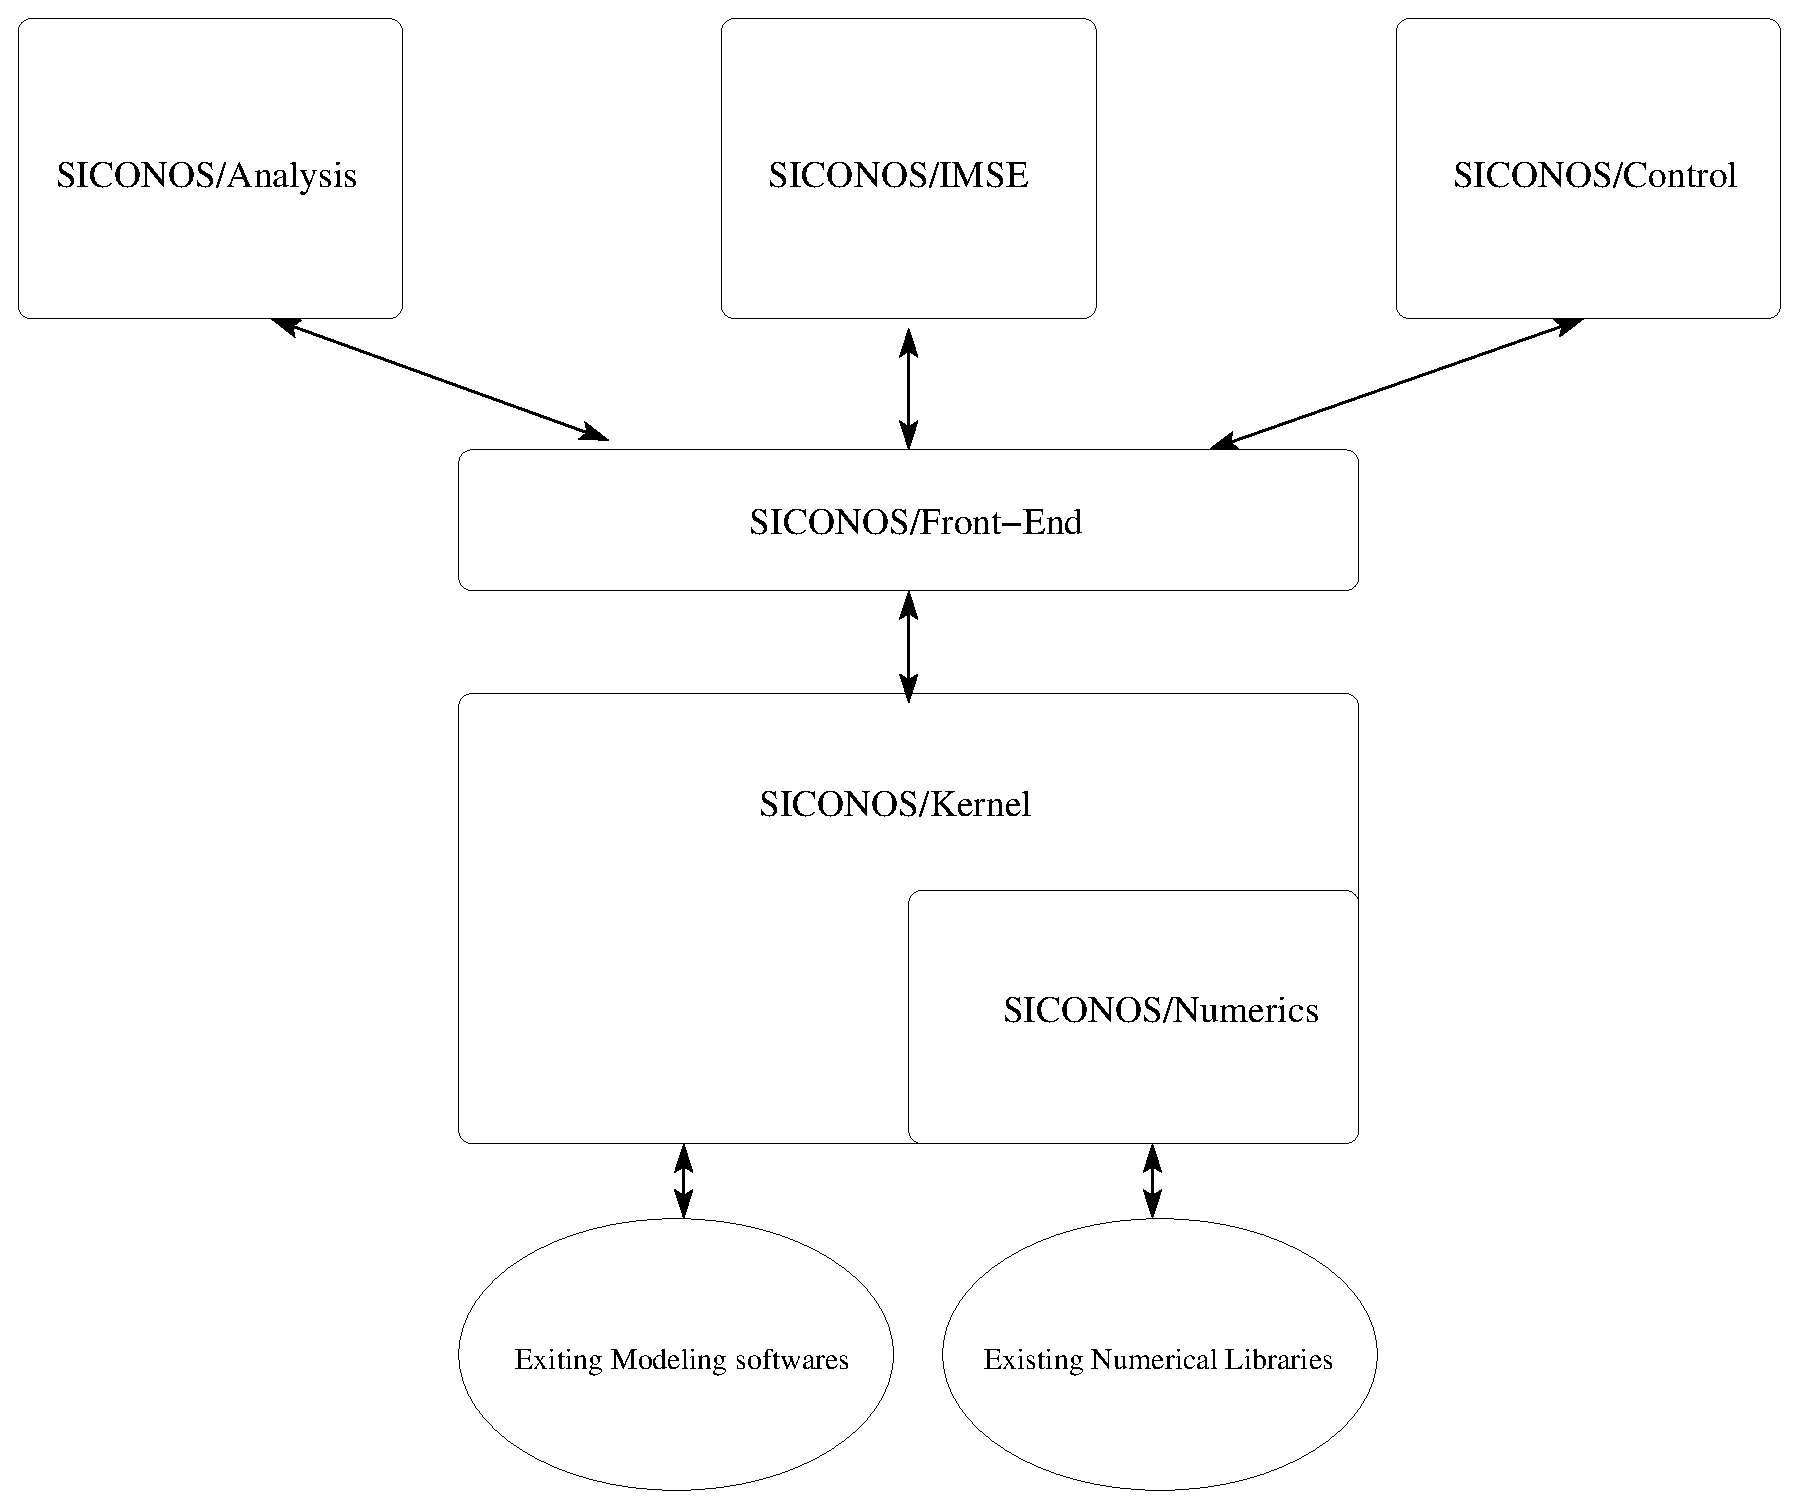
\includegraphics[width=0.7\textwidth]{./figure/functionalities.eps}
  \caption{Overview of the six functionalities of the \ac{siconos} Platform}
  \label{Fig:SICONOS-func}
\end{figure*}
\clearpage


\subsection{\acs{numerics}. Low-level numerical tools}
\label{Sec:SICONOS/Numerics}
This module will provide classes and methods to instantiate algebraic objects (vector, matrix, ...), 
with various storage formats (full, band, skyline ...). \\

This module has to perform various numerical functionalities~:
\begin{itemize}
 \item Linear algebra: linear system, eigenvalue, svd, ... \footnote{see LAPACK},
 \item Solver for non linear algebraic equation (Newton's method, ...),
 \item Solver for non smooth algebraic equation, (Generalized Newton Method, ...)
 \item Time integrator, ie basic computation for smooth time integration (one step integration, ...)
 \item Numerical, analytical or automatic differentiation,
 \item Mathematical programming (LCP, QP, optimization, ...).
\end{itemize}
%% \begin{ndrva}
%%   Doit on gerer les degres de liberte des integrateurs en temps dans Numerics ou dans Engine ? 
%% \end{ndrva}
\subsection{\acs{kernel}. Modelling and Simulation tools}
\label{Sec:SICONOS/Engine}



This module has to perform several major functionalities of the \ac{siconos} software. This module address  the modelling and the simulation  one physical process view as a non smooth dynamical system.


The functionalities of this module may be stated as follows:
\begin{enumerate}
\item \textbf{Model Formalization} :
  \begin{itemize}
  \item Define and describe several canonical model for general \ac{nsds}
    \begin{itemize}
    \item Linear complementarity systems (LCS)
    \item Lagrangian dynamical system with constraints
    \item Piecewise Smooth systems
    \item Higher order sweeping process
    \item Projected dynamical systems
    \item Unilateral differential inclusions
    \item Differential variational inequalities
    \item Discrete time system
    \end{itemize}
Several \ac{nsds} listed above (e.g LCS) may be decomposed in a smooth dynamical system, a set of relations between input/output variables and the state variables and a set of Non Smooth law which are listed below.
  \item Define and describe several canonical model for smooth dynamical systems SDS and the boundary conditions (IVP, BVP, ...)
    \begin{itemize}
    \item Linear Time invariant System (LTI)
    \item Non Linear System
    \item Lagrangian system
    \item Implicit System and differential Algebraic system
    \end{itemize}
  \item Define and describe several canonical model for relations between input/output variables and the state variables.
    \begin{itemize}
    \item Linear Time invariant relation
    \item Lagrangian relations (Jacobian)
    \item Non linear relations             \ldots
    \end{itemize}
  \item Define and describe several canonical model for non smooth Law
    \begin{itemize}
    \item Complementarity problem
    \item Relay system
    \item Friction-type law, etc.
    \end{itemize}
  \item Formalization of input systems into canonical model (general \ac{nsds}, SDS, Relations and non smooth laws)
  \item Analysis of coherence of the input systems 
  \item Translation between the  canonical models (general \ac{nsds}, SDS, and non smooth laws)
  \item Interface with description model tools (Plug-ins)(Existing modelling software, C F77 function, \ac{matlab} or \ac{scilab} function )
  \end{itemize}

\item  \textbf{Numerical strategies}
A numerical strategy is not only a set of basic numerical methods. It comprises the reformulation and the organization of the canonical model provided by the formalization part to realize the numerical computation. A numerical strategy is composed of :
  \begin{itemize}
  \item A time integrator method : Time--stepping or Event--Driven schemes.
  \item Evaluation or prediction of relations at discrete time. 
  \item Formalization of a one-step basic problem (LCP, QP, etc ...).
  \item Choice of a numerical method for solving the one step problem.   
  \item Interface with \ac{siconos}/numerics.
  \item Input/ Output of specific parameters for numerical strategies.
  \end{itemize}
\item  \textbf{Data representation and Save/Restart} The \ac{siconos} platform works with its own internal data structure, stored in the various attributes of the instantiated objects.  This internal data structure will consist of :
  \begin{itemize}
  \item data for the model formalization,
  \item data for the numerical strategy.
  \end{itemize}
Therefore, a specific storage structure  must be defined and constitutes the  \ac{siconos} specific files. This storage structure has to be very close to the object oriented data structure. The use of \ac{xml} and associated tools (DOM) seems  impossible to circumvent. 

If the \ac{siconos} specific files do not contain the complete representation of the formalized model, it needs to specify how to construct this representation, i.e. the name of the plug-in and the identifier of the data files for this plug-in.


Indeed, there are 3 ways to inform the internal data structure :
\begin{itemize}
\item The complete representation of the problem is loaded by reading \ac{siconos} specific and self-contained files. This way corresponds to a stand alone use of the platform.
\item The complete representation of the problem is loaded partially by reading \ac{siconos} specific files. In order to complete the missing part, the user has to provide the information using the API in interactive mode (object--oriented scripting language or the \ac{xxxlab} interface).
\item The complete representation of the problem is given by mixed files : external files describing the physical problem and its state and \ac{siconos} specific files describing the  model formalization and the numerical strategy. This way corresponds to a mixed use of the platform, in combination with an external software.
\end{itemize}

There are 2 ways to save the internal data structure :
\begin{itemize}
\item Using the \ac{siconos} specific and self-contained files,
\item Using mixed files: \ac{siconos} specific files and files saved by the external software.
\end{itemize}

Furthermore, the structure of the \ac{siconos} specific files must be able to represent all the above way to read and to save the data. It means that even for a mixed representation, the location of the external files must be specified in the \ac{siconos} specific files. 

Using these various mechanisms of reading and saving data, one can translate storage structure from external files to \ac{siconos} specific files.

This files must be exhaustive to allow a backup and a restart of a simulation at any specified time.  

The Engine must allow the user to trace internal variables during a simulation. These values of the internal variables could be exported in various formats for other post-processing softwares.

\end{enumerate}



%% \begin{ndrva}
%%   Mettre une figure de ce module. Tous les aspects pr�sents sur la figure doivent tre expliquer dans le texte.
%% \end{ndrva}

\subsection{\acs{frontend} }
\label{Sec:SICONOS/Front-End}

This module addresses the interface between the user and the platform. This interface have to fulfill several tasks :
\begin{itemize}
  \item To drive(command) the platform, i.e, to design a strategy of simulation,
  \item To provide an high-level language (logical tests, loops, \ldots),
  \item To be able to manage some basic mathematical computations,
  \item To provide informations to complete the data structure of the \ac{siconos}/Engine in interactive mode,
  \item To load external functions.
\end{itemize}


This Front-End will be realized by two APIs :
\begin{itemize}
\item A C++ API used through an object--oriented scripting language, 
\item An \ac{xxxlab} API used through \ac{xxxlab}. 
\end{itemize}




\subsection{\acs{control}.}
\label{Sec:SICONOS/Control}


The  major functionalities of the \ac{siconos}/Control  module are of the following :
\begin{itemize}
\item Validation of control strategies for \ac{nsds}
\item Feedback control with observers for \ac{nsds}
\item Trajectory planning     
\item Optimal control with constraints on the state and/or on the input.
\end{itemize}

In fact, the \ac{siconos}/Control  module will be built as an external module based on the C++ API provided by the \ac{siconos}/Front-end.

\subsection{\acs{analysis}.}
\label{Sec:SICONOS/Analysis}


This module  concerns the analysis of non smooth dynamical systems.  It provides several functionalities~:
\begin{itemize}
\item To check existence or well posed criteria, if any,
\item To search particular types of solutions (Periodic, steady-state, equilibrium sets,\ldots)
\item To study the stability of solutions (stable and unstable manifold.)
\item To perform  critical point detection (bifurcation detection)
\item To perform parametric continuation (path following methods)
\end{itemize}

Like the previous one, the \ac{siconos}/Analysis  module will be built as an external module based on the C++ API provided by the \ac{siconos}/Front-end.

\subsection{\acs{imse}.}
\label{Sec:SICONOS/pre-post}
 This module provides a  modelling and visualization environment for the \ac{kernel} based an the C++ API. Such a graphical  user interface  is  not planed, yet.

\section{General overview of the platform}

The platform should be used at three different levels~:
\begin{itemize}
\item in a partial level, using only the \ac{siconos}/Numerics part. It should be used in a standalone or interfaced through \ac{xxxlab},
\item in a global level through the standalone or the \ac{xxxlab} interface,
\item in a nested level through the \ac{siconos}/Control or \ac{siconos}/Analysis toolboxes.
\end{itemize}


\begin{sidewaysfigure}
  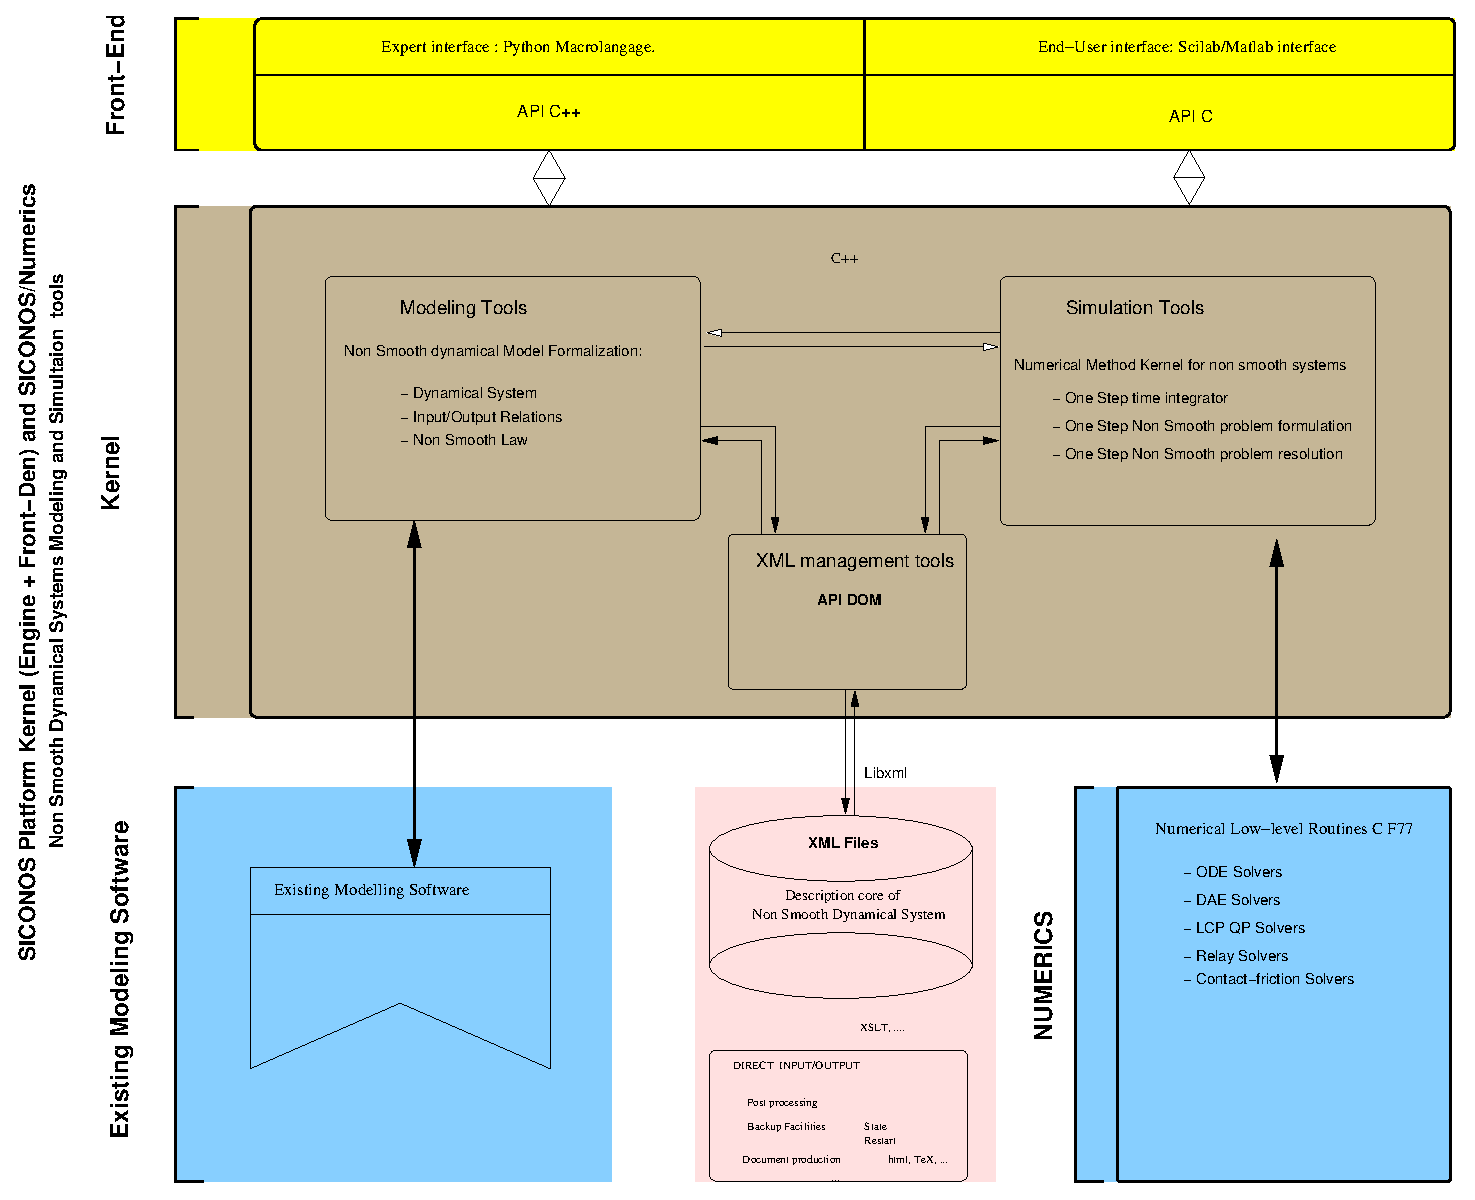
\includegraphics[width=0.8\textwidth]{./figure/Spec-v4.eps}
\end{sidewaysfigure}

\clearpage


%  use cases
\subsection{Users of the platform}

Three kind of users has been identified :
\begin{itemize}
\item End user : simplys uses the platform to run "basic"simulations.
\item Expert user : uses th platform to run simulations, but is also able to develop plugins with its own computation methods.
\item Developer : can add to the platform new features.
\end{itemize}.

%Diagramme d,utilisation general :
\begin{figure}[hb]
\begin{center}
\includegraphics[scale=0.65, bb=30 324 500 830, clip]{use_case_high_level.eps}
\end{center}
\caption{General use case}
\label{Fig:General use case}
\end{figure}

To get more details about the major features for each kind of users, see \ac{esd}.


%%%%%%%%%%%%%%%%%%%%%%%%%%%%%




\subsection{Flow-charts}

%\begin{ndrva}
%  Some flow charts will be interesting.  Goal: to fix ideas about the role of the modules and their relative independence.
%\end{ndrva}
The figure \ref{Fig:general_function} shows that it is possible to use external
application file (like \ac{lmgc90} file) via a dedicated plugin. An \ac{xml} plugin will
be provided to read \ac{xml} file.
The platform extracts some values from the simulation, and at the end of the
simulation, or at given steps of the simulation, the platform save the complet
state of the system in an \ac{xml} file. If we use this file as an input of the platform, we can restart the simulation at this point. 

\begin{figure}[hb]
\begin{center}
\includegraphics[angle=270, scale=0.85]{figure/GeneralFunctionning.eps}
\end{center}
\caption{General Functioning and files used}
\label{Fig:general_function}
\end{figure}
%%% Local Variables: 
%%% mode: latex
%%% TeX-master: "../report"
%%% End: 
